% sage_latex_guidelines.tex V1.20, 14 January 2017

\documentclass[Afour,sageh,times]{sagej}

\usepackage{moreverb,url}
\usepackage{cite}
\usepackage{amsmath}

%\usepackage{hyperref}
%\hypersetup{
%    colorlinks=true,
%    linkcolor=blue,
%    filecolor=magenta,      
%    urlcolor=cyan,
%}

\usepackage{listings}
\usepackage{xcolor}
%New colors defined belowC-FROST
\definecolor{codegreen}{rgb}{0,0.6,0}
\definecolor{codegray}{rgb}{0.5,0.5,0.5}
\definecolor{codepurple}{rgb}{0.58,0,0.82}
\definecolor{backcolour}{rgb}{0.95,0.95,0.92}
%Code listing style named "mystyle"
\lstdefinestyle{mystyle}{
  backgroundcolor=\color{backcolour},   commentstyle=\color{codegreen},
  keywordstyle=\color{magenta},
  numberstyle=\tiny\color{codegray},
  stringstyle=\color{codepurple},
  basicstyle=\ttfamily\footnotesize,
  breakatwhitespace=false,         
  breaklines=true,                 
  captionpos=b,                    
  keepspaces=true,                 
  numbers=left,                    
  numbersep=5pt,                  
  showspaces=false,                
  showstringspaces=false,
  showtabs=false,                  
  tabsize=2
}

%"mystyle" code listing set
\lstset{style=mystyle}
 
\urlstyle{same}

\usepackage[colorlinks,bookmarksopen,bookmarksnumbered,citecolor=red,urlcolor=red]{hyperref}
\newcommand\BibTeX{{\rmfamily B\kern-.05em \textsc{i\kern-.025em b}\kern-.08em
T\kern-.1667em\lower.7ex\hbox{E}\kern-.125emX}}

\def\volumeyear{2019}

\begin{document}

\runninghead{Tamali and Mekhfi}

\title{The new concept for a 3D digitisation system for 
\itshape{hostile environments}}

\author{TAMALI Mohammed\affilnum{1}, TAMALI Abderrahmane\affilnum{2}\\ and MEKHFI Soumia\affilnum{2}}

\affiliation{\affilnum{1}Faculty of Technology,Department of Electrical Engineering, SimulIA Team/ENERGARID Lab., PO Box 417, Algeria\\
\affilnum{2}Faculty of Technology, Department of Electrical Engineering, PO Box 417, Algeria}

\corrauth{TAMALI Mohammed, Faculty of TC-FROSTechnology,Department of Electrical Engineering, SimulIA Team/ENERGARID Lab., PO Box 417, Algeria}

\email{mtamali@gmail.com}

\begin{abstract}
Our project represents a contribution to the so-called” hostile” site management solution such as historic ruins, oil pipelines, earthquake-affected buildings, unexploited mines, sewage pipelines, sites infected by radioactivity. These places have a significant characteristic, the difficulty of access, which makes human intervention very expensive and dangerous. Our approach is to design a robotised autonomous and remote-controlled \citep{Winkler2009} vehicle \citep{Rohmer2013},\citep{Silva2007} on which a mounted remote sensing device LiDAR perform investigative and survey work.  The  LIDAR  works  in2D/3D digitisation to collect the data of the studied place and to transmit them then using different telecommunication means \citep{Rubenstein2012}. As a result of this operation, We conclude a 2D/3D map following the reception of the encrypted and sent images.  Technicians can, therefore, launch interventions within minimised risks \citep{Sprawitz2014}.\citep{Bendjedid2016}.
\end{abstract}

\keywords{Robotics, Hostile site, 3D digitisation, Point-Cloud, LiDAR, Transmission}

\maketitle
\section{Introduction}
Several techniques help humans in their environment, including those difficult, repetitive, or painful spots. In the concept of these techniques, we will focus ideas on robotics. This one defines all the methods allowing the modelling and the realisation of the robots \citep{Krichmar2001}. The usage of these machines, such as:
\begin{enumerate}
    \item In an industry (industrial robotics - Car construction and hostile tasks)
    \item In a domestic environment (domestic robotics, home surveillance, automation)
    \item In medical (Medical Robotics
    \item Assisted Surgery, teleoperation, Care during the war)
    \item For the military field (Military Robotics-UAV, Missile, Drone, ...)
    \item Moreover, even robotics in hostile environments.
\end{enumerate}
By their name, hostile environments do not allow humans to intervene efficiently in a particular context. Among these environments, we will find places of past explosions, places of nuclear exploitation (dangerous effect), planets, the threatened historic ruins, and even the areas affected by an earthquake or a volcano. In these different cases, robotics responds to the need \citep{Yahya2017} for manipulation or management of remote processes because of potential dangers and the harmfulness caused by the presence of the man on the spot.

The primary aspect of character recognition of the place is essential to know. Some other things are essential to consider, such as the evaluation of the rates of difficulty, the stability of the environment, the degrees of freedom, and other parameters. We consider them so that we can ask the robot well-adapted characteristics and compatible, as much as possible, with the desired medium as tasks for robots in hostile environments. Also in sanitary and wastewater circulation systems where their function is to discover the blocking points of and maintain excellent continuity, In times of war, the robot be sacrificed to advance on mined places and consequently invalidate them. While the space robot makes a trip from the earth to a planet for a specific study, equipped to be able to confront, virtually, any type of event and must be able to face it. In terms of the field of health, a robot can access into a human body and do internal operations without the practical need for openness and as a result of potential complications.

Such systems allow interactivity with surrounding environments by using means well adapted to take information or to apply actions after treatment.
A robot is forced to use essential means \citep{Okamura2004}, such as communication with the human supervisor, a motor for the displacement, energy for power supply, and complementary means for regular operation.

The choice of system peripherals depends on several environmental parameters such as weather conditions (temperature, pressure and other environmental conditions), hostile character, range and degree of visibility, and on-board telecommunication possibilities.
Take the case of historical ruins (Fig.\ref{fig:hammad}) or places after an earthquake (Fig.\ref{fig:earthquake}), the use of LiDAR for navigation requires knowledge of the environment surrounding the system and to know the geographical dimensions to be able to move and perform specific tasks.
To transferring data related to the 3D acquisition of the hostile sites, we refer to the use of different ways for communication purposes such as GSM networks (Internet or SMS), Wifi transmission, or ZigBee. A camera for remote control is more than required. Finally, the shape of the robot system is security for the continuity of tasks.
Speaking of people's lives (case of earthquakes) or access to challenging environments allows to review the cost of intervention by humans and risks to cash, for this reason, we qualify, the use of a machine as an alternative to qualitatively reduce the cost of the operation.

\section{Site characterised as hostile}
By definition, a hostile environment is an environment in which the human being is subject to physical aggression (pressure, noise, temperature, radiation, or chemical).
Huge costs are paid each year to meet the needs of repeated interventions on the sewage network (29216 interventions on 1125 township according to ONA -Water National Office- in 2018), The heritage Fouggara in the city of Adrar (Fig.\ref{fig:Reggane}) dies a day in a day for lack of rehabilitation as the Ksour of the great south of Algeria.
The French nuclear tests of the 1960s would kill even today in Algeria in Reggane especially (according to sputnik-news 01/2019), The radioactivity affected according to the experts Southern Europe and all North Africa.
The Ministry of Tourism, Culture, and Environment launches special programs to help spaces potentially exploitable by a national tourist action. Most of these spaces are now in ruins, say inaccessible (Casbah (Fig.\ref{fig:Casba}), Ksour of the North, Ksar of Kenadsa and Taghit to Bechar, Ksar of Tamentit to Adrar), The untapped mine of Kenadsa and its wasteland currently represents a significant challenge, to the development of the city of Kenadsa (Fig.\ref{fig:Kendsa}). The socioeconomic impact exceeds the capacity, in short, of Algeria and calls upon the international contribution.

\begin{figure}
    \centering
    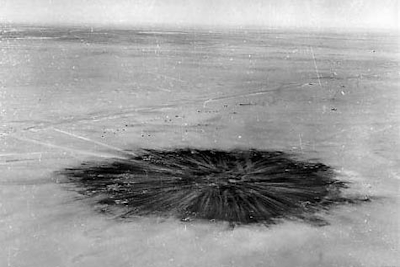
\includegraphics[scale=15]{RagganeNuclear.png}
    \caption{Area substantially infected with nuclear radiation, Reggane-Adrar, Algeria}
    \label{fig:Reggane}
\end{figure}

\subsection{Literature (etymological) definition}
In biology, the environment can say together external factors that act permanently or permanently on an animal, a plant, a biocenosis and to which the organisms must be adapted to survive and perpetuate themselves.
In chemistry and physics: the medium can determine a substance in which a reaction occurs, a phenomenon which is characterised by specific properties (for example, acidic medium).
Hostile: is an adjective, which seems contrary to the man and his companies. He can also define aggression.
So the hostile environment is defined as an environment in which the man life is subject to physical aggression such as pressure, temperature, or radiation.

\subsection{Technical definition}
A hostile environment is a place where moving and operating intuitively on complicated and challenging terrain and even interactivity safely with that environment is a challenge.
The hostile site defines a localised environment in which risks on human life is high due to physical aggression such as mechanical, pressure, temperature, radiation or electrical.
A hostile environment is a place where moving and operating intuitively on complicated and challenging terrain and even interactivity safely with that environment is a challenge.

The complexity of this site can be characterised either by the terrain of displacement in speaking on obstacles, the existence in this environment can be harmful or risky, and we can also say on a hostile environment the place of which a situation in an environment that is too complicated to tame or manage well.
Here are some illustrations that show hostile backgrounds:
\begin{figure}
    \centering
    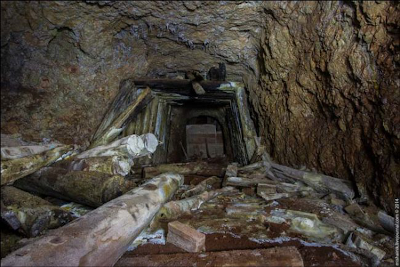
\includegraphics[scale=15]{KenadsaMine.png}
    \caption{Abandoned mine of Kenadsa Bechar, Algeria}
    \label{fig:Kendsa}
\end{figure}
\begin{figure}
    \centering
    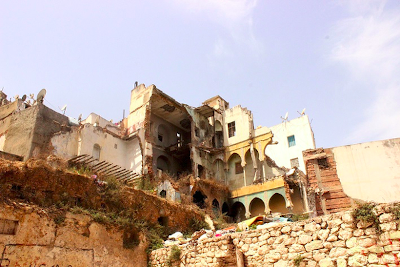
\includegraphics[scale=15]{Casba.png}
    \caption{Ruins of historical Casba in Algiers, Algeria}
    \label{fig:Casba}
\end{figure}
\begin{figure}
    \centering
    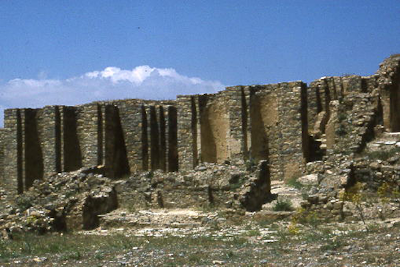
\includegraphics[scale=15]{Qal'abaniHammad.png}
    \caption{Historic Qal'a of Bani Hammad at Bejaia, Algeria}
    \label{fig:hammad}
\end{figure}
\begin{figure}
    \centering
    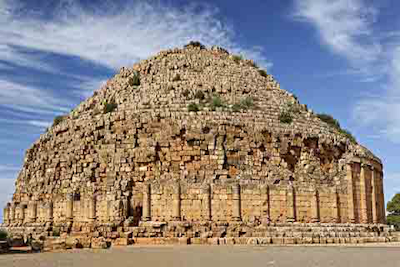
\includegraphics[scale=15]{Moretany.png}
    \caption{Royal Mausoleum of Mauretania At Sidi Rached-Near Algiers, Algeria}
    \label{fig:mauretania}
\end{figure}
\begin{figure}
    \centering
    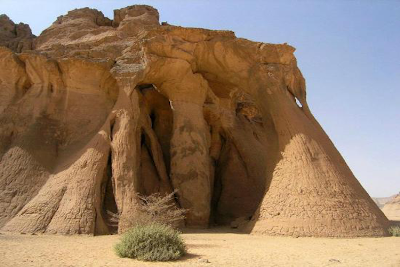
\includegraphics[scale=15]{tassili.png}
    \caption{National Park At Tassili n'Ajjer, Algeria}
    \label{fig:Tassili}
\end{figure}
\begin{figure}
    \centering
    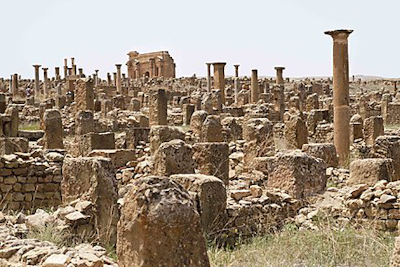
\includegraphics[scale=15]{Timgad.png}
    \caption{Timgad-Roman Ruins At Aures region, Algeria}
    \label{fig:Timgad}
\end{figure}

\subsection{Some statistics}
For UNESCO, ruin is a construction which has lost so much of its original form and substance that its loss of potential unity as a functional structure. We still understand, a non-functional built object.
A ruin is not welcome in most cities today, where the safety of traffic and production seems prohibited. As a result, the ruins are often destroyed and erased from the urban environment. However, the ruins have authentic functions, in particular, identity and, in some cases, the actors of the urban planning decided to maintain them, to preserve them, even to highlight them.
Sometimes the ancient place rests a great difficulty with the drilling and excavation and remains unworkable or abandoned, for example, many points in the pyramids in Egypt because of the dangers emanating.
In Algeria, there is an exceptional number of historical relics, the history of Algeria is rich, namely the evidence of the passage of civilisations (Byzantine, Roman and Ottoman), also the period of the French colonisation.

According to the United Nations Educational, Scientific and Cultural Organisation, statistics highlight places considered as the most damaged heritage sites in Algeria.
From 1992 to 2010 (Fig.11), statistics were harmful; the number of earthquakes with sensible magnitude has increased by 10. The impact on building and industrial organisations reached a level never seen before.

\begin{figure}
    \centering
    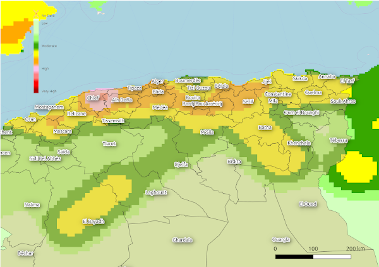
\includegraphics[scale=25]{EarthQuakeStat.png}
    \caption{Site affected by earthquake with sensible magnitude, Algeria}
    \label{fig:earthquake}
\end{figure}

The intervention work in these hostile sites, costs big sums of money, finding, which pushes us to devote more attention to the negatively impacted investments.
The losses are even more expensive if they relate to the lives of the maintenance technicians in the places of intervention.
Strong demand, behind significant investments, for the manufacture of equipment adapted to the total or partial intervention in the hostile places considered. Our approach is in this context, and the goal is to develop a robotic vehicle for digital 3D recognition of these places. This acquisition of information will benefit stakeholders in time and cost, and even more in the risks to lives.

\section{Our approach}
For any design, it is better to join the ideas a methodology of realisation. This action defines a sequence of well-known steps.
In the current context of our paper, it is asked to think \citep{Oudeyer2004}, draw and realise a physical object, to digitise in three dimensions (3D), a place qualified as hostile.
So, the characteristics of the requirements described by the research, make that the search for a justified approach is in favour of the tool, that we will think/use/transform for purposes of 3D digitisation.
Many solutions of the same kind exist with more or less fallout. The great concern is on the side of the prices which, the more the effect is required, the more the price is high. The challenge comes back to the demand for a solution of lower taxes with comparable efficiency.
In this context, we have highlighted a solution, allowing, from a 2D planar LiDAR to obtain a complete 3D data of the place to study (Fig.\ref{fig:RealisedLiDAR3D}).

\begin{figure}
    \centering
    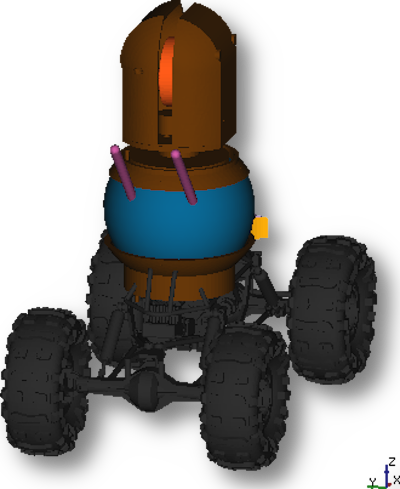
\includegraphics[scale=15]{robot.png}
    \caption{Our Approach (back view).}
    \label{fig:back_view}
\end{figure}
\begin{figure}
    \centering
    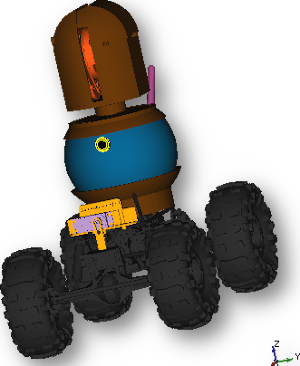
\includegraphics[scale=20]{robot1.png}
    \caption{Our Approach (front view).}
    \label{fig:front_view}
\end{figure}

\begin{figure}
    \centering
    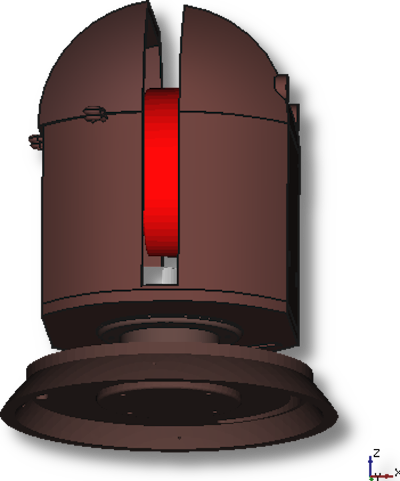
\includegraphics[scale=15]{lidar3d.png}
    \caption{The LiDAR 3D model (FreeCAD Drawing).}
    \label{fig:LiDAR3D}
\end{figure}
\begin{figure}
    \centering
    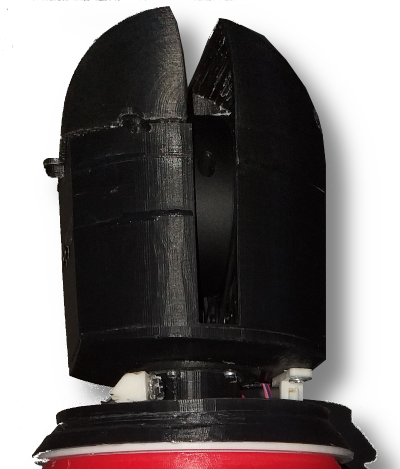
\includegraphics[scale=15]{lidar3dprntd.png}
    \caption{The LiDAR 3D model (The 3D printed LiDAR).}
    \label{fig:3DprintedLiDAR}
\end{figure}

\begin{figure}
    \centering
    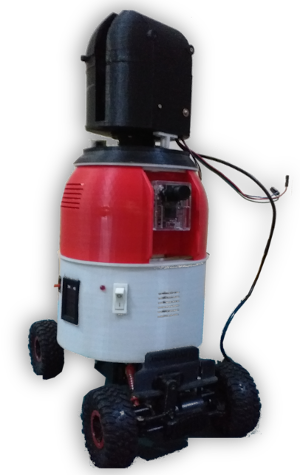
\includegraphics[scale=16]{robot3.png}
    \caption{Realised Test Robot with LiDAR3D mounted.}
    \label{fig:RealisedLiDAR3D}
\end{figure}

The target prototype developed, overcomes one of the high complexity, the optimal position of the acquisition element concerning the rest of the body of the robot vehicle. The following figures clearly show the meaning of this judgement. Four proposed variants exist, the four figures  \ref{fig:Model1-HX-Swinging}, \ref{fig:Model2-VZ-Swinging}, \ref{fig:Model3-HY-Swinging} and \ref{fig:Model4-HZ-LinearMoving} will explain this idea.

\begin{figure}
    \centering
    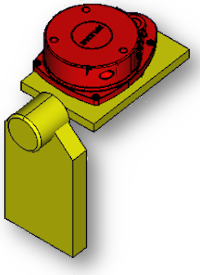
\includegraphics[scale=25]{model1.png}
    \caption{Available configurations (HX-Swinging).}
    \label{fig:Model1-HX-Swinging}
\end{figure}
\begin{figure}
    \centering
    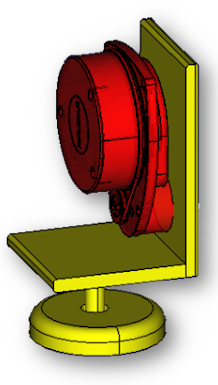
\includegraphics[scale=1.5]{model2.png}
    \caption{Available configurations (VZ-Swinging).}
    \label{fig:Model2-VZ-Swinging}
\end{figure}
\begin{figure}
    \centering
    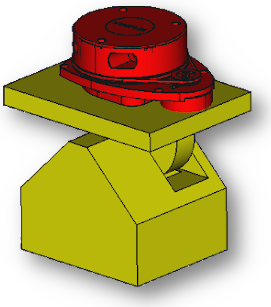
\includegraphics[scale=1.5]{model3.png}
    \caption{Available configurations (HY-Swinging).}
    \label{fig:Model3-HY-Swinging}
\end{figure}
\begin{figure}
    \centering
    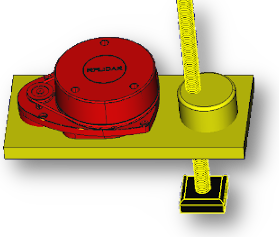
\includegraphics[scale=2]{model4.png}
    \caption{Available configurations (HZ-Linear Moving).}
    \label{fig:Model4-HZ-LinearMoving}
\end{figure}

Practically, each configuration has advantages and disadvantages, in particular, the coverage, that make the scanning device touch particular and unique geometry of the hostile areas \citep{Kaminaga2016}. Generally, the horizontal versions are subjects of compulsory swing in order to scan the 3D space while that with swinging or vertical movements acquire mechanical possibilities in addition to the horizontal versions.
The LiDAR must swing thousands of times, for a given task, to finalise a 3D map of the place to acquire.
Likewise, vertical configurations favour an optimal scan in the direction required by hostile environments.
Under these conditions, we adopted the configuration 2 (Fig.\ref{fig:Model2-VZ-Swinging}), with vertical sway around the Z axis.

\begin{figure}
    \centering
    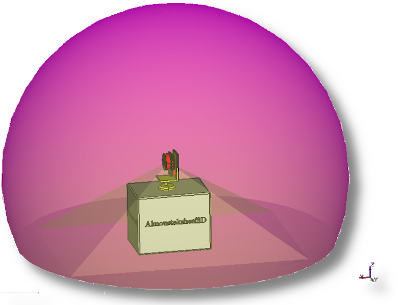
\includegraphics[scale=1.5]{limit2.png}
    \caption{Scope and coverage of the second config.}
    \label{fig:Limitationofthesecondconfig}
\end{figure}

\subsection{The characteristics of the hostile places}
Hostile environnment are the most, an area \citep{Strabala2013}, \citep{Cully2015}, \citep{DAndola2018}, that many essential details are found, practically in all the directions. Which implies, the use of equipment adapted to scrutinise this type of details. The second configuration is very feasible and favourable while it implies to hostile site criteria.

The ETH laboratory in Zurich has developed a robot machine called ANYmal East whose characteristics are of the order of the criteria and requirements of hostile environments.
Our target reference is to meet the majority of criteria \citep{Kolling2016} than those guaranteed by ANYmal (Fig.\ref{fig:RobotANYmal}) or Cheetah (Fig.\ref{fig:RobotCheetah}). The following list lists the said criteria:

\begin{itemize}
    \item Adjustable design profile \citep{Duquette2008}
    \item Essential Payload
    \item Efficient tools for acquiring hostile sites \citep{Drotman2017},\citep{Boumediene2012}
    \item Optimum energy autonomy \citep{Kim2010}
    \item Adequate software base \citep{Quigley2009},\citep{EnriqueFernandezLuisSanchezCrespoAnilMahtani2015},\citep{Kortenkamp2008},\citep{mtamali2006}
    \item Modular design \citep{Indicated1987}
    \item Collaboration and Multitask \citep{Dahl2009},\citep{Parker2009},\citep{Rekleitis2001}
    \item Navigation system and re-adaptable mobility \citep{Handfield2002}
    \item Data transmission compatible with the tasks \citep{Gerkey2004}
    \item Control and Supervision \citep{Geng2009}, \citep{Hahnel2003}
\end{itemize}

\begin{figure}
    \centering
    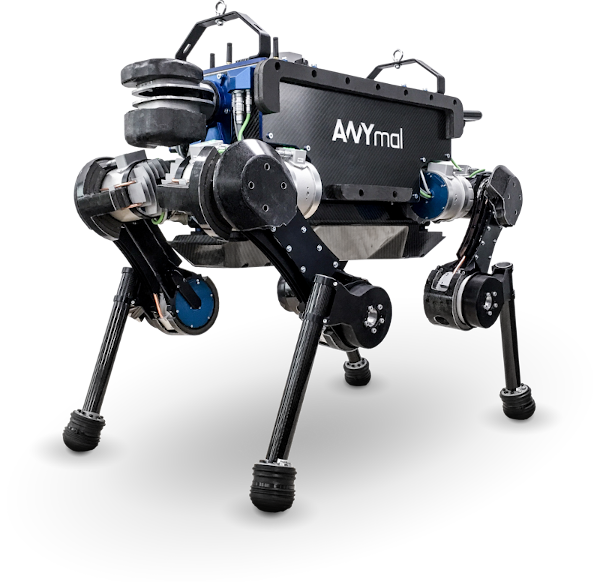
\includegraphics[scale=0.4]{ANYmal-Bedi-1030x999.png}
    \caption{Robot ANYmal, ETH/Robotics \citep{Cully2015},\citep{Hwangbo2019},\citep{Yahya2017}.}
    \label{fig:RobotANYmal}
\end{figure}
\begin{figure}
    \centering
    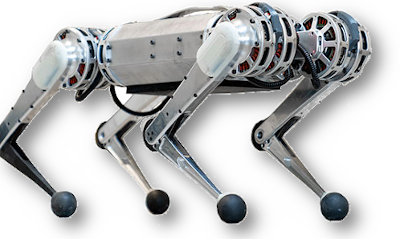
\includegraphics[scale=1.2]{mit-cheetah.png}
    \caption{Robot Cheetah, MIT \citep{Seok2013},\citep{DiCarlo2018},\citep{Li2014}}
    \label{fig:RobotCheetah}
\end{figure}
The general structure on which our model was developed and practically executed is illustrated by the following overall scheme:
\begin{figure}
    \centering
    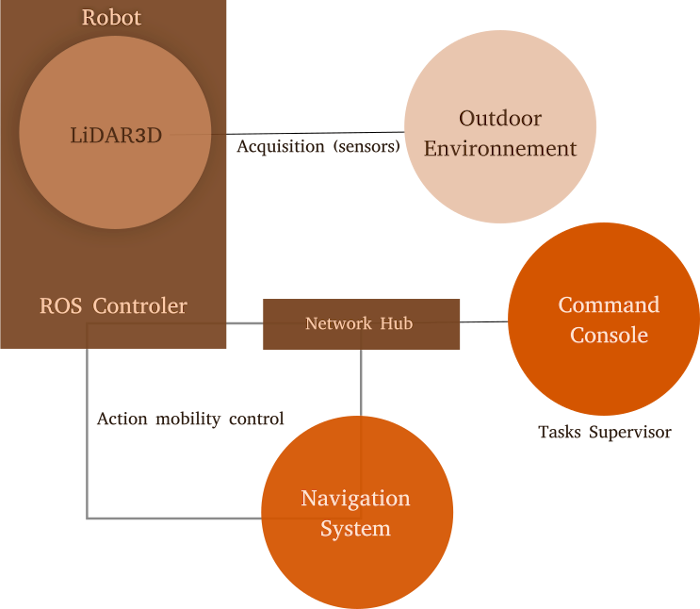
\includegraphics[scale=32]{GeneralAspect.png}
    \caption{The General aspect of our purpose}
    \label{fig:GeneralAspect}
\end{figure}
Any estimate made, our design remains valid for a 3D acquisition of places whose hostility is much tainted by geometric characteristics difficult to inaccessible.
The size of our robot, its payload and more particularly, the LiDAR3D used are sensitive parameters for the design of quality and undoubted efficiency.

\section{Methodology and Results}
The robot AL Moustaksheef 3D is an automatic machine characterised, from the dynamic point of view, by the mobility on the spot, by three degrees of freedom. The resulting movements provide the robot with the ability to move forward/backwards on four wheels and thus turn to clear paths safely inland usually not regular.
As a displacement aid, the Odometry function (OpenMV Smart Camera) can present images in addition to a specific processing of shapes and colours recognition. The choice of modification of the axis of displacement is also possible by the use of a servomotor which will let the robot turn left or right.
In this first attempt, the Navigation / Odometry system pair is in its basic version. The integration and extension of an extension are made easy under ROS (Robot Operating System).
The element overcoming the body can swing around its vertical axis so that the LiDAR can scan a given place.
These abilities can be further developed to allow other degrees of freedom DDL to the robot.
The AL Moustaksheef 3D robot overhang on a chassis. On which a body surmounted by the LiDAR 3D acquisition system. This requirement requires the coupling of equipment of characteristics compatible with the request.

To meet this arrangement, we adopt specific equipment for the assembly of the robot. For the essential part, in this case, the 3D acquisition, SAMSUNG Artik 710 module is chosen as the main element connected to a ROBOPEACK brand LiDAR equipment well known for its stability and its qualities.
The main characteristic of Laser of the acquisition module is maximum efficiency distance of up to eight meters, which is valid compared to the mission to be assigned (3D acquisition of hostile environments).
The second essential module is that of navigation that allows the robot to move on trajectories (In standalone mode or remote control) in hostile places. Finally, the Control / Command module links the robot and its outside world via a certain number of means of radio connection (WiFi, Bluetooth, ZigBee or GSM).
The equipment and micro-controller cards used are around an RPLiDAR A1M8 from ROBOPEACK managed by an ARTIK 710 with a complementary accessories.
Based on the technical specifications of the manufacturer Robopeack, we have written an additional code to translate the data acquired in 2D as 3D images, following a geometric re-projection from Polar 2D to Cartesian 3D.
The RPLiDAR Lidar works in horizontal 2D. Our transformation consisted of its rotation on a vertical plane, rotate.

\begin{figure}
    \centering
    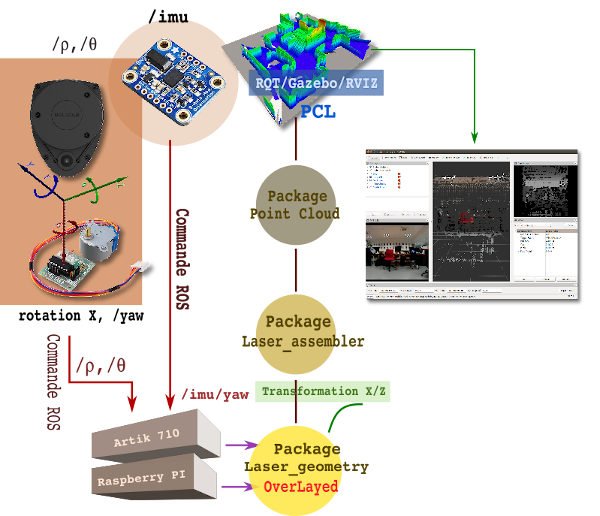
\includegraphics[scale=0.3]{scan.png}
    \caption{The 2D to 3D LiDAR transformation concept}
    \label{fig:3dlidar}
\end{figure}

For the software part, ROS is a flexible and Open-Source software framework for programming robots. ROS provides a hardware abstraction layer in which developers can create robotic applications without worrying about the underlying hardware. ROS also provides various software tools to view and debug a robot's data. The heart of the ROS framework is a Middleware messaging system in which processes can communicate and exchange data with each other, even when running from different machines. The transmission of ROS messages can be synchronous or asynchronous.

The software in ROS is organised as packages and offers functional modularity and re-usability. Using the hardware abstraction layer and the ROS messaging middleware, developers can create a multitude of robotic features, such as mapping and navigation (in mobile robots). Almost all the features of ROS will be agnostic so that all kinds of robots can use it. New robots can directly use this capability packet without modifying any code inside the package.
ROS has many collaborations in universities, and many developers contribute to it.
For the software part, We follow a specific methodology. LiDAR is a conception of the firm Robopeak, and this company makes available to its customers, an SDK accessible via the site slamware.com. This library offers all the firmware and development tools to take control of the hardware. The SDK is a multi-platform application, so we can install it on any machine that supports an operating system.
Robopeak, based on the SDK as RPLiDAR A1M8 driver, proposes a ROS package projecting the use of LiDAR as a ROS component. The corresponding ROS node is accessible as the PUBLISHER \textbf{/scan} transmitter node. The data is exploitable, at will, under the name of the topic \textbf{/scan}. At this level, it is recommended to transcribe the extracted data in Cartesian $(x,y,z)$, since they are in polar $(\rho,\theta)$.

The ROS Laser\_geometry package can respond to this first task by projecting in polar coordinates values on a Cartesian axis system. At the output, the data are the same except that this time they are in Cartesian representation. The following laser\_assembler package makes it possible, among other things, to collect a large number of acquisitions in the form of a PCL Cloud (Point Cloud) that can be used later for purely graphic reasons.
In parallel, the gyro-meter helps to know the positions and angles concerning the magnetic north. This last device is used through the RTIMUlib library as a gyro-meter driver and the RTIMULib\_ROS package to publish vital information, \textbf{/imu/yaw}, to 3D digitisation.
Indeed, without this information, it is challenging to extract 3D from 2D without knowledge of information on the situations of the scanned points but on a projection $Z$.
Besides, the laser\_assembler package can collect double information \textbf{/scan} and \textbf{/imu/yaw} to make Cartesian projection $(x,y,z)$ and output a PCL (Point Cloud2) result. At this stage, the visualisation is necessary on an interface compatible with the PCL format, and it is the turn of the tools of the system \textbf{ROS} \citep{Quigley2009}, \textbf{RQT} \citep{Kumar2016}, \textbf{RVIZ} \citep{Hernandez-Mendez2018}, \citep{DaveHershbergerDavidGossow2009}, \citep{Omara2016}, \citep{Shen2018}, \citep{Arvind2016} or \textbf{GAZEBO} \citep{Meyer2012}, \citep{Joseph2015}, \citep{Zhang2015}, \citep{Afanasyev2015}, \citep{Rosa2015}. In what follows, we will discuss the need for visualisation and its focus on a single interface such as a dashboard.

\begin{figure}
    \centering
    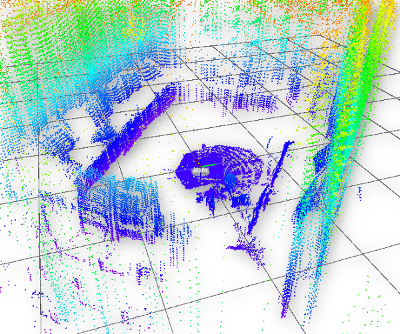
\includegraphics[scale=20]{scan1.png}
    \caption{Sample of 3D scanning}
    \label{fig:3dscan}
\end{figure}

For the record, The ROS system project was launched in 2007 at Stanford University under the name switchyard. Later, in 2008, the development was undertaken by Start-Up robotic research called Willow Garage. The leading development in ROS that happened in Willow Garage \url{http://www.willowgarage.com/}. In 2013, Willow Garage researchers formed the Open Source Robotic Foundation (OSRF) \url{http://www.osrfoundation.org/}. ROS is actively maintained and updated by OSRF so far.
The main transformation formula used in addition to the package Laser\_geometry was the common tool well-known:

\begin{equation} \label{eq1}
\begin{bmatrix}
\phi \\ \theta \\ \psi 
\end{bmatrix}=
    \begin{bmatrix}
        Arctan(\frac{2(q_0.q_1+q_2.q_3)}{1-2(q_1^2+q_2^2)})\\
        Arcsin\left(2(q_0.q_2-q_3.q_1) \right)\\
        Arctan(\frac{2(q_0.q_3+q_1.q_2)}{1-2(q_2^2+q_3^2)})
    \end{bmatrix}
\end{equation}

The reading of the result indicates to us that the moving object on which the mounted gyro-meter, balances relative to the axes with the angles $\phi, \theta, \psi$ corresponding to the Quaternion:

\begin{equation}\label{eq2}
\begin{bmatrix}
  x: 0.559329092503\\
  y: 0.51973170042\\
  z: 0.468855112791\\
  w: -0.444077640772
\end{bmatrix}
\end{equation}

The submitted values are not readily exploitable in this format, and it is necessary to proceed to a change of representation Quaternion to Euler $\phi, \theta, \psi$ by the equation \ref{eq1}.\newline
For the ROS system, the \textbf{tf} package contains \textit{Quat-Euler} or \textit{Euler-Quat} conversion procedures. For a python program, we will use, for example:

\begin{lstlisting}[language=Python, caption=Python code for conversion Quat to Euler]
    #!/usr/bin/env python
    import rospy
    from sensor_msgs.msg import Imu
    from tf.transformations import euler_from_quaternion, quaternion_from_euler
    def get_Euler (msg):
        global roll, pitch, yaw
        orientation_q = msg.pose.pose.orientation
        orientation_list = [orientation_q.x, orientation_q.y, orientation_q.z, orientation_q.w]
        (roll, pitch, yaw) = euler_from_quaternion (orientation_list)
        print "roll, pitch, yaw : %f, %f, %f" % (roll, pitch, yaw)
    rospy.init_node('quaternion_to_euler')
    sub = rospy.Subscriber ('/imu', Imu, get_Euler)
    r = rospy.Rate(10)
    while not rospy.is_shutdown():
        r.sleep()
\end{lstlisting}

\begin{figure}
    \centering
    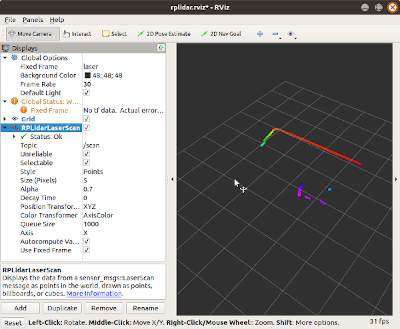
\includegraphics[scale=20]{result3.png}
    \caption{2D scanning sample, without transformation}
    \label{fig:2dscanWtoutConv}
\end{figure}

Graphical interfacing is the best \textbf{HMI} \textit{(Human Machine Interface)} means \citep{Kumar2016}, necessary to make the results more readable compared to the primary data considered. In this context, several tools are available, the distinction or the adoption of one of them still guided by the number of Plugins/AddOns it offers separately from other platforms of the same category.

\begin{figure}
    \centering
    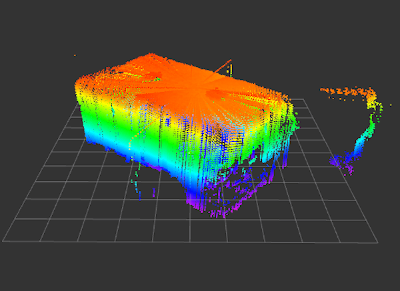
\includegraphics[scale=20]{Resultat1.png}
    \caption{PCL 3D digitisation with Z Height based color}
    \label{fig:Resultat1}
\end{figure}
\begin{figure}
    \centering
    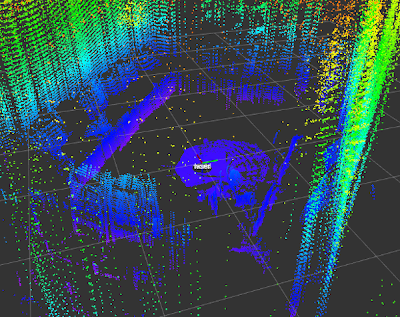
\includegraphics[scale=20]{Resultat3.png}
    \caption{3D digitisation with Z Height based Color}
    \label{fig:Resultat3}
\end{figure}

\section{Conclusion}
The growing development of mobile telecommunications and \textbf{IoT} technologies have made the robots have been integrated into applications as diverse as they are useful and standard, in-home automation, in industrial applications for the remote control and monitoring of complex systems but also in the security of systems, defence and protection of the territories, goods and people. Moreover, about the progress made, the words of our project, mention autonomous/remote control robots which are primarily designed to provide help with tedious tasks, and for ease of work with forced characters and which can take time and costs money.\newline
In our project, we devoted ourselves to the development of a robot that allows us to explore hostile or dangerous areas without taking risks. These places are difficult to access, which makes human intervention very expensive on the lives to save, and equipment to use.
Our realisation consists in designing a remote-controlled robot based on a sensing device 'LiDAR3D' working in digitisation and 3D scanning in order to recover the data of the studied place and to transmit them employing telecommunication media.\newline
In this project, we forged our skills on more than one axis:

\begin{itemize}
    \item The technical methodologies of designing a proper prototype.
    \item Technical drawings on specialised software and, consequently, the 3D printer runs.
    \item Managing various assemblies involving various types of equipment.
    \item The setup and testing of the prototype made, in this case, the robot we named 'AL Moustaksheef 3D'.
\end{itemize}
As a perspective, we stayed targeting some improvements in future works by extending the geometry, mechanic issues, electronic or process limitations encountered.

\bibliographystyle{SageH}
\bibliography{mybib.bib}

\end{document}
